\documentclass[twoside]{book}

% Packages required by doxygen
\usepackage{fixltx2e}
\usepackage{calc}
\usepackage{doxygen}
\usepackage[export]{adjustbox} % also loads graphicx
\usepackage{graphicx}
\usepackage[utf8]{inputenc}
\usepackage{makeidx}
\usepackage{multicol}
\usepackage{multirow}
\PassOptionsToPackage{warn}{textcomp}
\usepackage{textcomp}
\usepackage[nointegrals]{wasysym}
\usepackage[table]{xcolor}

% NLS support packages
\usepackage[bahasa]{babel}
% Font selection
\usepackage[T1]{fontenc}
\usepackage[scaled=.90]{helvet}
\usepackage{courier}
\usepackage{amssymb}
\usepackage{sectsty}
\renewcommand{\familydefault}{\sfdefault}
\allsectionsfont{%
  \fontseries{bc}\selectfont%
  \color{darkgray}%
}
\renewcommand{\DoxyLabelFont}{%
  \fontseries{bc}\selectfont%
  \color{darkgray}%
}
\newcommand{\+}{\discretionary{\mbox{\scriptsize$\hookleftarrow$}}{}{}}

% Page & text layout
\usepackage{geometry}
\geometry{%
  a4paper,%
  top=2.5cm,%
  bottom=2.5cm,%
  left=2.5cm,%
  right=2.5cm%
}
\tolerance=750
\hfuzz=15pt
\hbadness=750
\setlength{\emergencystretch}{15pt}
\setlength{\parindent}{0cm}
\setlength{\parskip}{0.2cm}
\makeatletter
\renewcommand{\paragraph}{%
  \@startsection{paragraph}{4}{0ex}{-1.0ex}{1.0ex}{%
    \normalfont\normalsize\bfseries\SS@parafont%
  }%
}
\renewcommand{\subparagraph}{%
  \@startsection{subparagraph}{5}{0ex}{-1.0ex}{1.0ex}{%
    \normalfont\normalsize\bfseries\SS@subparafont%
  }%
}
\makeatother

% Headers & footers
\usepackage{fancyhdr}
\pagestyle{fancyplain}
\fancyhead[LE]{\fancyplain{}{\bfseries\thepage}}
\fancyhead[CE]{\fancyplain{}{}}
\fancyhead[RE]{\fancyplain{}{\bfseries\leftmark}}
\fancyhead[LO]{\fancyplain{}{\bfseries\rightmark}}
\fancyhead[CO]{\fancyplain{}{}}
\fancyhead[RO]{\fancyplain{}{\bfseries\thepage}}
\fancyfoot[LE]{\fancyplain{}{}}
\fancyfoot[CE]{\fancyplain{}{}}
\fancyfoot[RE]{\fancyplain{}{\bfseries\scriptsize Dibangkitkan pada tanggal Kamis 19 Maret 2015 11\+:15\+:12 untuk Kalkulator Sakti oleh Doxygen }}
\fancyfoot[LO]{\fancyplain{}{\bfseries\scriptsize Dibangkitkan pada tanggal Kamis 19 Maret 2015 11\+:15\+:12 untuk Kalkulator Sakti oleh Doxygen }}
\fancyfoot[CO]{\fancyplain{}{}}
\fancyfoot[RO]{\fancyplain{}{}}
\renewcommand{\footrulewidth}{0.4pt}
\renewcommand{\chaptermark}[1]{%
  \markboth{#1}{}%
}
\renewcommand{\sectionmark}[1]{%
  \markright{\thesection\ #1}%
}

% Indices & bibliography
\usepackage{natbib}
\usepackage[titles]{tocloft}
\setcounter{tocdepth}{3}
\setcounter{secnumdepth}{5}
\makeindex

% Hyperlinks (required, but should be loaded last)
\usepackage{ifpdf}
\ifpdf
  \usepackage[pdftex,pagebackref=true]{hyperref}
\else
  \usepackage[ps2pdf,pagebackref=true]{hyperref}
\fi
\hypersetup{%
  colorlinks=true,%
  linkcolor=blue,%
  citecolor=blue,%
  unicode%
}

% Custom commands
\newcommand{\clearemptydoublepage}{%
  \newpage{\pagestyle{empty}\cleardoublepage}%
}


%===== C O N T E N T S =====

\begin{document}

% Titlepage & ToC
\hypersetup{pageanchor=false,
             bookmarks=true,
             bookmarksnumbered=true,
             pdfencoding=unicode
            }
\pagenumbering{roman}
\begin{titlepage}
\vspace*{7cm}
\begin{center}%
{\Large Kalkulator Sakti \\[1ex]\large 0.\+1 }\\
\vspace*{1cm}
{\large Dibangkitkan oleh Doxygen 1.8.9.1}\\
\vspace*{0.5cm}
{\small Kamis 19 Maret 2015 11:15:12}\\
\end{center}
\end{titlepage}
\clearemptydoublepage
\tableofcontents
\clearemptydoublepage
\pagenumbering{arabic}
\hypersetup{pageanchor=true}

%--- Begin generated contents ---
\chapter{Indeks Namespace}
\section{Daftar Namespace}
Berikut ini daftar namespace yang didokumentasikan, dengan keterangan singkat\+:\begin{DoxyCompactList}
\item\contentsline{section}{\hyperlink{namespaceMemori}{Memori} \\*Kelas yang digunakan untuk merepresentasikan ekspresi, merupakan pembungkusan vector of (pointer to token) }{\pageref{d4/dd4/namespaceMemori}}{}
\item\contentsline{section}{\hyperlink{namespaceMenghitung}{Menghitung} \\*Kelas yang digunakan untuk melakukan proses menghitung token }{\pageref{df/d37/namespaceMenghitung}}{}
\item\contentsline{section}{\hyperlink{namespaceParser}{Parser} \\*Kelas yang digunakan untuk merepresentasikan bilangan arab }{\pageref{d3/d71/namespaceParser}}{}
\item\contentsline{section}{\hyperlink{namespaceSTL}{S\+T\+L} \\*Kelas exception spesifik class stack }{\pageref{d5/da1/namespaceSTL}}{}
\end{DoxyCompactList}

\chapter{Indeks Hierarki Kelas}
\section{Hierarki Kelas}
Hierarki kelas ini diurutkan kurang-\/lebih berdasarkan abjad\+:\begin{DoxyCompactList}
\item \contentsline{section}{Bilangan\+Exception}{\pageref{classBilanganException}}{}
\item \contentsline{section}{Calculator}{\pageref{classCalculator}}{}
\item \contentsline{section}{Calculator\+Exception}{\pageref{classCalculatorException}}{}
\item \contentsline{section}{Expression}{\pageref{classExpression}}{}
\item \contentsline{section}{Memori}{\pageref{classMemori}}{}
\item \contentsline{section}{stack$<$ T $>$\+:\+:node}{\pageref{structstack_1_1node}}{}
\item \contentsline{section}{Parser}{\pageref{classParser}}{}
\item \contentsline{section}{Parser\+Exception}{\pageref{classParserException}}{}
\item \contentsline{section}{Penghitung}{\pageref{classPenghitung}}{}
\item \contentsline{section}{Penghitung\+Exception}{\pageref{classPenghitungException}}{}
\item \contentsline{section}{stack$<$ T $>$}{\pageref{classstack}}{}
\item \contentsline{section}{Stack\+Exp}{\pageref{classStackExp}}{}
\item \contentsline{section}{Token}{\pageref{classToken}}{}
\begin{DoxyCompactList}
\item \contentsline{section}{Bilangan}{\pageref{classBilangan}}{}
\begin{DoxyCompactList}
\item \contentsline{section}{Arab}{\pageref{classArab}}{}
\item \contentsline{section}{Romawi}{\pageref{classRomawi}}{}
\end{DoxyCompactList}
\item \contentsline{section}{Operator}{\pageref{classOperator}}{}
\item \contentsline{section}{Perintah}{\pageref{classPerintah}}{}
\end{DoxyCompactList}
\item \contentsline{section}{vector$<$ T $>$}{\pageref{classvector}}{}
\item \contentsline{section}{vector$<$ Expression $>$}{\pageref{classvector}}{}
\item \contentsline{section}{vector$<$ Token $\ast$ $>$}{\pageref{classvector}}{}
\end{DoxyCompactList}

\chapter{Indeks Struktur Data}
\section{Struktur Data}
Berikut ini daftar struktur data, dengan penjelasan singkat\+:\begin{DoxyCompactList}
\item\contentsline{section}{\hyperlink{classArab}{Arab} \\*Class \hyperlink{classArab}{Arab} }{\pageref{d0/d70/classArab}}{}
\item\contentsline{section}{\hyperlink{classBilangan}{Bilangan} \\*Class \hyperlink{classBilangan}{Bilangan} }{\pageref{d2/dac/classBilangan}}{}
\item\contentsline{section}{\hyperlink{classBilanganException}{Bilangan\+Exception} \\*Class \hyperlink{classBilanganException}{Bilangan\+Exception} }{\pageref{da/dd3/classBilanganException}}{}
\item\contentsline{section}{\hyperlink{classCalculator}{Calculator} \\*Class \hyperlink{classCalculator}{Calculator} }{\pageref{d8/dbe/classCalculator}}{}
\item\contentsline{section}{\hyperlink{classCalculatorException}{Calculator\+Exception} \\*Class \hyperlink{classCalculatorException}{Calculator\+Exception} }{\pageref{df/d30/classCalculatorException}}{}
\item\contentsline{section}{\hyperlink{classExpression}{Expression} \\*Class \hyperlink{classExpression}{Expression} }{\pageref{de/d94/classExpression}}{}
\item\contentsline{section}{\hyperlink{classMemori}{Memori} \\*Class \hyperlink{classMemori}{Memori} }{\pageref{df/df7/classMemori}}{}
\item\contentsline{section}{\hyperlink{classOperator}{Operator} }{\pageref{d4/dad/classOperator}}{}
\item\contentsline{section}{\hyperlink{classParser}{Parser} }{\pageref{d0/d40/classParser}}{}
\item\contentsline{section}{\hyperlink{classParserException}{Parser\+Exception} }{\pageref{df/d55/classParserException}}{}
\item\contentsline{section}{\hyperlink{classPenghitung}{Penghitung} }{\pageref{d3/dd5/classPenghitung}}{}
\item\contentsline{section}{\hyperlink{classPenghitungException}{Penghitung\+Exception} }{\pageref{d1/de8/classPenghitungException}}{}
\item\contentsline{section}{\hyperlink{classPerintah}{Perintah} }{\pageref{d9/de7/classPerintah}}{}
\item\contentsline{section}{\hyperlink{classRomawi}{Romawi} }{\pageref{d9/de3/classRomawi}}{}
\item\contentsline{section}{\hyperlink{classstack}{stack$<$ T $>$} \\*Class stack }{\pageref{d1/dc2/classstack}}{}
\item\contentsline{section}{\hyperlink{classStackExp}{Stack\+Exp} }{\pageref{d8/d10/classStackExp}}{}
\item\contentsline{section}{\hyperlink{classToken}{Token} }{\pageref{d2/d6e/classToken}}{}
\item\contentsline{section}{\hyperlink{classvector}{vector$<$ T $>$} \\*Class vector }{\pageref{d7/dfc/classvector}}{}
\end{DoxyCompactList}

\chapter{Dokumentasi Namespace}
\hypertarget{namespaceMemori}{}\section{Referensi Namespace Memori}
\label{namespaceMemori}\index{Memori@{Memori}}


Kelas yang digunakan untuk merepresentasikan ekspresi, merupakan pembungkusan vector of (pointer to token).  




\subsection{Keterangan Lengkap}
Kelas yang digunakan untuk merepresentasikan ekspresi, merupakan pembungkusan vector of (pointer to token). 

Kelas yang digunakan untuk menyimpan list ekspresi.

\begin{DoxyAuthor}{Penulis}
Ibrohim Kholilul Islam 
\end{DoxyAuthor}
\begin{DoxyVersion}{Versi}
0.\+1 
\end{DoxyVersion}
\begin{DoxyDate}{Tanggal}
Maret 2015 
\end{DoxyDate}
\begin{DoxyWarning}{Peringatan}
semua pointer token yang diberikan dapat ditunjuk oleh lebih dari 1 ekspresi. 

destructor tidak bertangung jawab kepada token yang diberikan.
\end{DoxyWarning}
\begin{DoxyAuthor}{Penulis}
Ibrohim Kholilul Islam 
\end{DoxyAuthor}
\begin{DoxyVersion}{Versi}
0.\+1 
\end{DoxyVersion}
\begin{DoxyDate}{Tanggal}
Maret 2015 
\end{DoxyDate}
\begin{DoxyWarning}{Peringatan}
Pada destructor, semua token yang terdapat pada ekspresi dihapus. 
\end{DoxyWarning}

\hypertarget{namespaceMenghitung}{}\section{Referensi Namespace Menghitung}
\label{namespaceMenghitung}\index{Menghitung@{Menghitung}}


Kelas yang digunakan untuk melakukan proses menghitung token.  




\subsection{Keterangan Lengkap}
Kelas yang digunakan untuk melakukan proses menghitung token. 

Kelas yang digunakan untuk melakukan proses exception penghitung.

\begin{DoxyAuthor}{Penulis}
Afrizal Fikri 
\end{DoxyAuthor}
\begin{DoxyVersion}{Versi}
0.\+1 
\end{DoxyVersion}
\begin{DoxyDate}{Tanggal}
Maret 2015 
\end{DoxyDate}
\begin{DoxyWarning}{Peringatan}
-\/ 
\end{DoxyWarning}

\hypertarget{namespaceParser}{}\section{Referensi Namespace Parser}
\label{namespaceParser}\index{Parser@{Parser}}


Kelas yang digunakan untuk merepresentasikan bilangan arab.  




\subsection{Keterangan Lengkap}
Kelas yang digunakan untuk merepresentasikan bilangan arab. 

Kelas abstrak yang digunakan untuk merepresentasikan token.

Kelas yang digunakan untuk merepresentasikan bilangan romawi.

Kelas yang digunakan untuk merepresentasikan token perintah.

Kelas yang digunakan untuk melakukan proses pembuatan execption dari parser.

Kelas yang digunakan untuk melakukan proses parsing string.

Kelas yang digunakan untuk merepresentasikan token operator.

Kelas exception spesifik class \hyperlink{classCalculator}{Calculator}.

Kelas utama kalkulator yang melakukan loop input-\/proses-\/output.

Kelas exception spesifik class \hyperlink{classBilangan}{Bilangan}.

Kelas Abstrak yang digunakan untuk merepresentasikan bilangan.

\begin{DoxyAuthor}{Penulis}
Satria Priambada 
\end{DoxyAuthor}
\begin{DoxyVersion}{Versi}
0.\+1 
\end{DoxyVersion}
\begin{DoxyDate}{Tanggal}
Maret 2015 
\end{DoxyDate}
\begin{DoxyWarning}{Peringatan}
-\/ 
\end{DoxyWarning}

\hypertarget{namespaceSTL}{}\section{Referensi Namespace S\+T\+L}
\label{namespaceSTL}\index{S\+T\+L@{S\+T\+L}}


Kelas exception spesifik class stack.  




\subsection{Keterangan Lengkap}
Kelas exception spesifik class stack. 

Kelas vector yang diimplementasi berdasarkan \hyperlink{namespaceSTL}{S\+T\+L} C++.

Kelas stack yang diimplementasi berdasarkan \hyperlink{namespaceSTL}{S\+T\+L} C++.

\begin{DoxyAuthor}{Penulis}
Afrizal Fikri 
\end{DoxyAuthor}
\begin{DoxyVersion}{Versi}
0.\+1 
\end{DoxyVersion}
\begin{DoxyDate}{Tanggal}
Maret 2015 
\end{DoxyDate}
\begin{DoxyWarning}{Peringatan}
-\/
\end{DoxyWarning}
\begin{DoxyAuthor}{Penulis}
Ibrohim Kholilul Islam 
\end{DoxyAuthor}
\begin{DoxyVersion}{Versi}
0.\+1 
\end{DoxyVersion}
\begin{DoxyDate}{Tanggal}
Maret 2015 
\end{DoxyDate}
\begin{DoxyWarning}{Peringatan}
-\/ 
\end{DoxyWarning}

\chapter{Dokumentasi Struktur Data}
\hypertarget{classArab}{}\section{Referensi Kelas Arab}
\label{classArab}\index{Arab@{Arab}}


Class \hyperlink{classArab}{Arab}.  




{\ttfamily \#include \char`\"{}Arab.\+h\char`\"{}}

Diagram hierarki kelas untuk Arab\+:\begin{figure}[H]
\begin{center}
\leavevmode
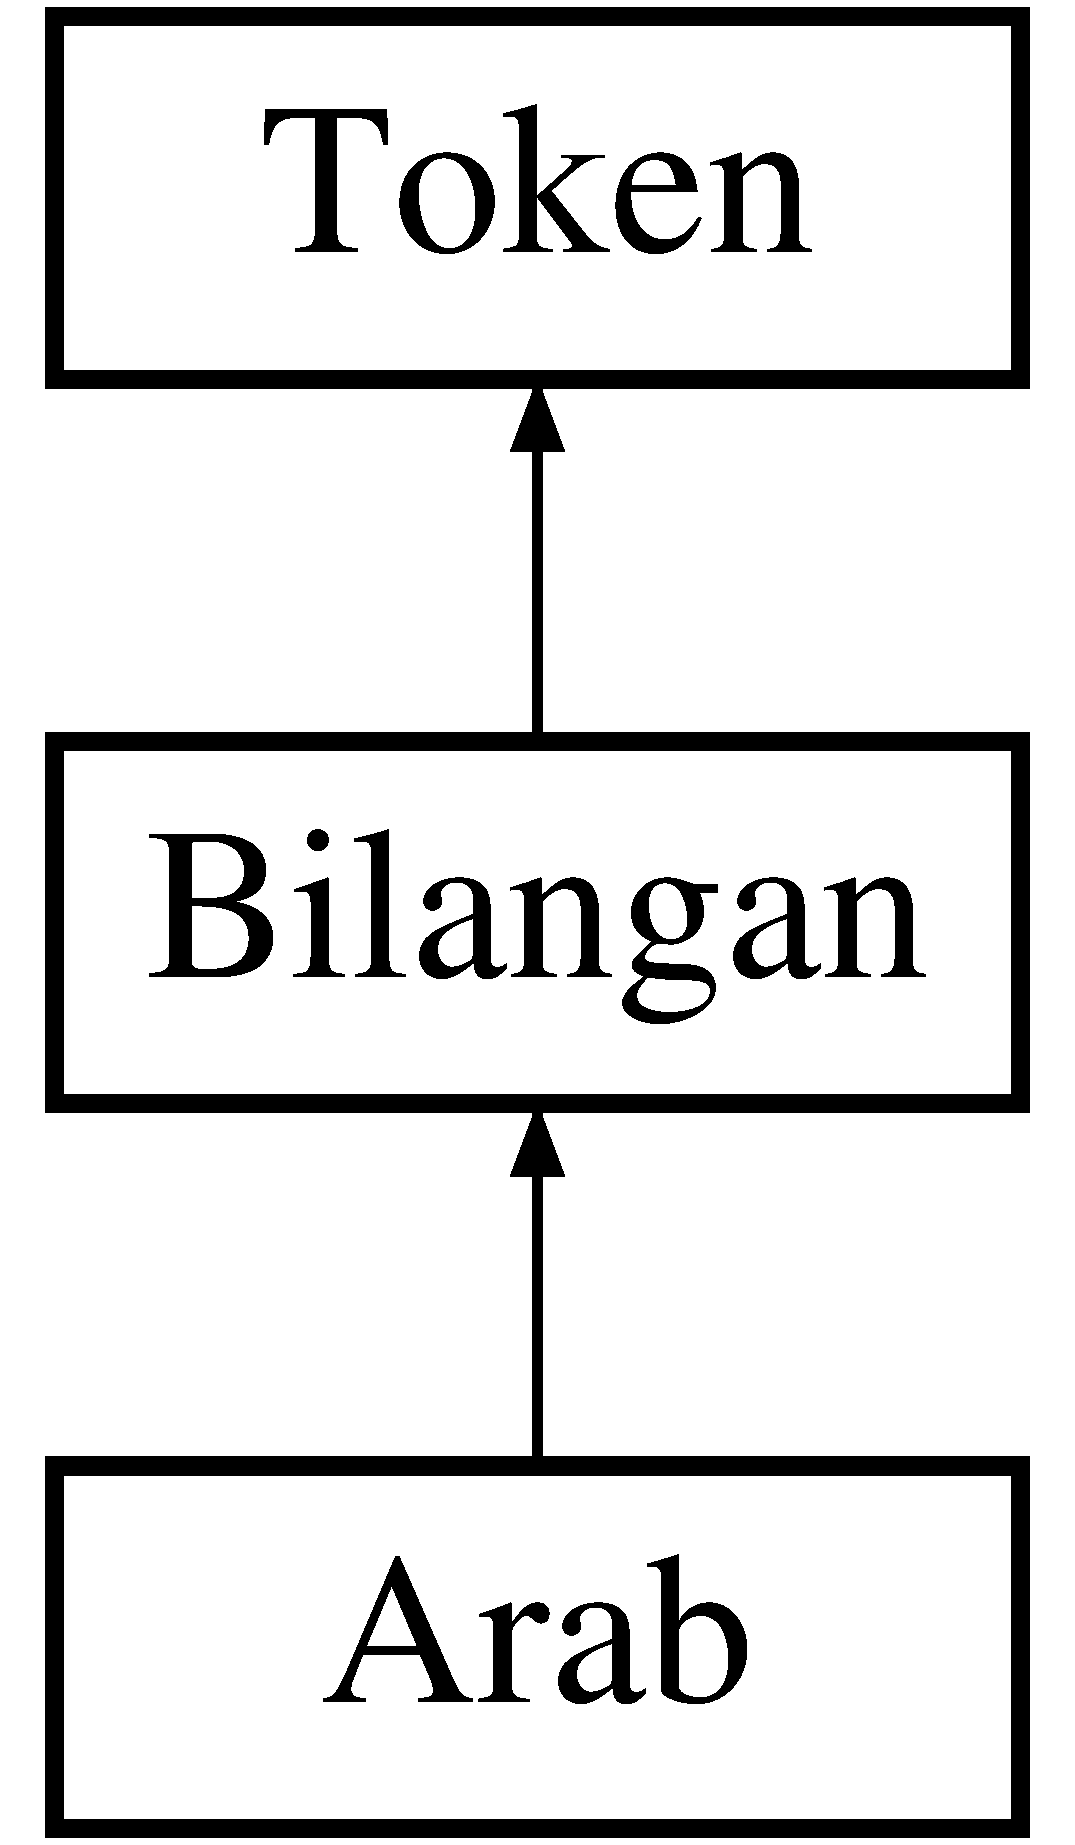
\includegraphics[height=3.000000cm]{d0/d70/classArab}
\end{center}
\end{figure}
\subsection*{Fungsi Anggota Publik}
\begin{DoxyCompactItemize}
\item 
\hyperlink{classArab_afdddf6ff9c7724ddb71c625db0847893}{Arab} ()
\begin{DoxyCompactList}\small\item\em Constructor default. \end{DoxyCompactList}\item 
\hyperlink{classArab_add184fe39f6fc81d20f5b26d4b9758a3}{Arab} (const double d)
\begin{DoxyCompactList}\small\item\em Constructor with parameter double. \end{DoxyCompactList}\item 
\hyperlink{classArab_a28e10b4e58b32730dce2a4f3f98a825e}{Arab} (const std\+::string \&s)
\begin{DoxyCompactList}\small\item\em Constructor with parameter string. \end{DoxyCompactList}\item 
\hyperlink{classArab_a2629b0540731753334ebb19161774f7a}{$\sim$\+Arab} ()
\begin{DoxyCompactList}\small\item\em Destructor. \end{DoxyCompactList}\item 
double \hyperlink{classArab_ac0fb43a1da728805bec9add68fd46fa0}{Get\+Value} ()
\begin{DoxyCompactList}\small\item\em Fungsi Get\+Value. \end{DoxyCompactList}\item 
std\+::string \hyperlink{classArab_a96e515d21840b8ddfe50414505618200}{Display} ()
\begin{DoxyCompactList}\small\item\em Fungsi Display. \end{DoxyCompactList}\end{DoxyCompactItemize}
\subsection*{Atribut Privat}
\begin{DoxyCompactItemize}
\item 
\hypertarget{classArab_a1f491a08c53d1f8b5450a0c8deefc1f4}{}double {\bfseries Value}\label{classArab_a1f491a08c53d1f8b5450a0c8deefc1f4}

\end{DoxyCompactItemize}


\subsection{Keterangan Lengkap}
Class \hyperlink{classArab}{Arab}. 

Kelas yang digunakan untuk merepresentasikan bilangan arab

cctor dan operator= tidak pernah dipakai 

\subsection{Dokumentasi Konstruktor \& Destruktor}
\hypertarget{classArab_afdddf6ff9c7724ddb71c625db0847893}{}\index{Arab@{Arab}!Arab@{Arab}}
\index{Arab@{Arab}!Arab@{Arab}}
\subsubsection[{Arab}]{\setlength{\rightskip}{0pt plus 5cm}Arab\+::\+Arab (
\begin{DoxyParamCaption}
{}
\end{DoxyParamCaption}
)}\label{classArab_afdddf6ff9c7724ddb71c625db0847893}


Constructor default. 

Konstruktor yang digunakan untuk membuat Objek arab dengan nilai 0 \hypertarget{classArab_add184fe39f6fc81d20f5b26d4b9758a3}{}\index{Arab@{Arab}!Arab@{Arab}}
\index{Arab@{Arab}!Arab@{Arab}}
\subsubsection[{Arab}]{\setlength{\rightskip}{0pt plus 5cm}Arab\+::\+Arab (
\begin{DoxyParamCaption}
\item[{const double}]{d}
\end{DoxyParamCaption}
)}\label{classArab_add184fe39f6fc81d20f5b26d4b9758a3}


Constructor with parameter double. 

Konstruktor yang digunakan untuk membuat Objek arab dengan nilai double yang diberikan


\begin{DoxyParams}{Parameter}
{\em d} & double \\
\hline
\end{DoxyParams}
\begin{DoxyPrecond}{Kondisi Awal}
d terdefinisi 
\end{DoxyPrecond}
\hypertarget{classArab_a28e10b4e58b32730dce2a4f3f98a825e}{}\index{Arab@{Arab}!Arab@{Arab}}
\index{Arab@{Arab}!Arab@{Arab}}
\subsubsection[{Arab}]{\setlength{\rightskip}{0pt plus 5cm}Arab\+::\+Arab (
\begin{DoxyParamCaption}
\item[{const std\+::string \&}]{s}
\end{DoxyParamCaption}
)}\label{classArab_a28e10b4e58b32730dce2a4f3f98a825e}


Constructor with parameter string. 

Konstruktor yang digunakan untuk membuat Objek arab dari nilai string yang diberikan


\begin{DoxyParams}{Parameter}
{\em s} & string \\
\hline
\end{DoxyParams}
\begin{DoxyPrecond}{Kondisi Awal}
s terdefinisi 
\end{DoxyPrecond}
\hypertarget{classArab_a2629b0540731753334ebb19161774f7a}{}\index{Arab@{Arab}!````~Arab@{$\sim$\+Arab}}
\index{````~Arab@{$\sim$\+Arab}!Arab@{Arab}}
\subsubsection[{$\sim$\+Arab}]{\setlength{\rightskip}{0pt plus 5cm}Arab\+::$\sim$\+Arab (
\begin{DoxyParamCaption}
{}
\end{DoxyParamCaption}
)\hspace{0.3cm}{\ttfamily [inline]}}\label{classArab_a2629b0540731753334ebb19161774f7a}


Destructor. 


\begin{DoxyParams}{Parameter}
{\em none} & \\
\hline
\end{DoxyParams}


\subsection{Dokumentasi Anggota\+: Fungsi}
\hypertarget{classArab_a96e515d21840b8ddfe50414505618200}{}\index{Arab@{Arab}!Display@{Display}}
\index{Display@{Display}!Arab@{Arab}}
\subsubsection[{Display}]{\setlength{\rightskip}{0pt plus 5cm}std\+::string Arab\+::\+Display (
\begin{DoxyParamCaption}
{}
\end{DoxyParamCaption}
)\hspace{0.3cm}{\ttfamily [virtual]}}\label{classArab_a96e515d21840b8ddfe50414505618200}


Fungsi Display. 

Fungsi untuk mendapatkan string untuk ditampilkan


\begin{DoxyParams}{Parameter}
{\em none} & \\
\hline
\end{DoxyParams}
\begin{DoxyReturn}{Mengembalikan}
string 
\end{DoxyReturn}


Mengimplementasikan \hyperlink{classBilangan}{Bilangan}.

\hypertarget{classArab_ac0fb43a1da728805bec9add68fd46fa0}{}\index{Arab@{Arab}!Get\+Value@{Get\+Value}}
\index{Get\+Value@{Get\+Value}!Arab@{Arab}}
\subsubsection[{Get\+Value}]{\setlength{\rightskip}{0pt plus 5cm}double Arab\+::\+Get\+Value (
\begin{DoxyParamCaption}
{}
\end{DoxyParamCaption}
)\hspace{0.3cm}{\ttfamily [virtual]}}\label{classArab_ac0fb43a1da728805bec9add68fd46fa0}


Fungsi Get\+Value. 

Fungsi untuk mendapatkan nilai dari \hyperlink{classBilangan}{Bilangan} \hyperlink{classArab}{Arab}


\begin{DoxyParams}{Parameter}
{\em none} & \\
\hline
\end{DoxyParams}
\begin{DoxyReturn}{Mengembalikan}
double 
\end{DoxyReturn}


Mengimplementasikan \hyperlink{classBilangan}{Bilangan}.



Dokumentasi untuk kelas ini dibangkitkan dari file berikut\+:\begin{DoxyCompactItemize}
\item 
/home/ibrohim/oop002/Arab.\+h\end{DoxyCompactItemize}

\hypertarget{classBilangan}{}\section{Referensi Kelas Bilangan}
\label{classBilangan}\index{Bilangan@{Bilangan}}


Class \hyperlink{classBilangan}{Bilangan}.  




{\ttfamily \#include \char`\"{}Bilangan.\+h\char`\"{}}

Diagram hierarki kelas untuk Bilangan\+:\begin{figure}[H]
\begin{center}
\leavevmode
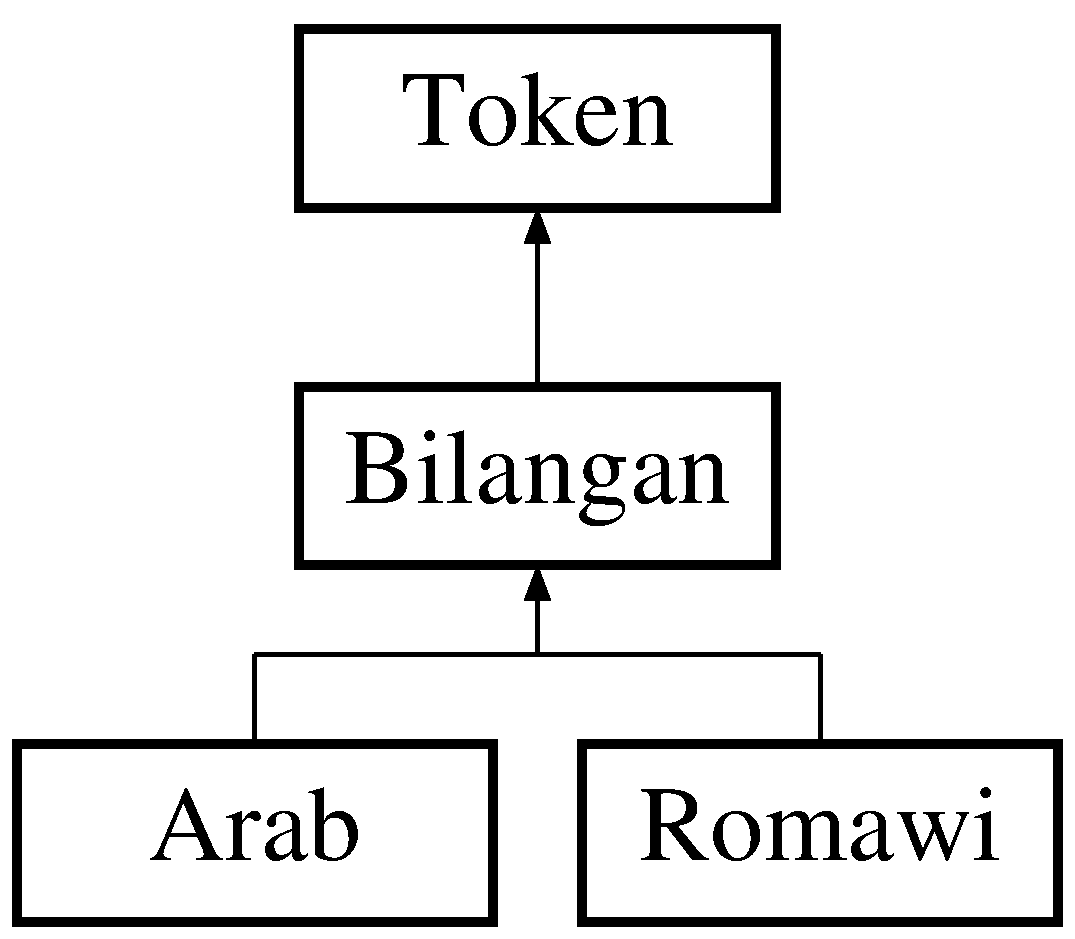
\includegraphics[height=3.000000cm]{d2/dac/classBilangan}
\end{center}
\end{figure}
\subsection*{Fungsi Anggota Publik}
\begin{DoxyCompactItemize}
\item 
\hypertarget{classBilangan_ab2ee8800f19568a48bf9cc7a2e74bc3d}{}virtual std\+::string {\bfseries Display} ()=0\label{classBilangan_ab2ee8800f19568a48bf9cc7a2e74bc3d}

\item 
\hypertarget{classBilangan_a3bf3d5edae1146c224521ffef88343a5}{}Enum\+Type {\bfseries Get\+Type} ()\label{classBilangan_a3bf3d5edae1146c224521ffef88343a5}

\item 
\hypertarget{classBilangan_a0e5aa4a90d3fe974e806f39ebbf813b9}{}virtual double {\bfseries Get\+Value} ()=0\label{classBilangan_a0e5aa4a90d3fe974e806f39ebbf813b9}

\end{DoxyCompactItemize}


\subsection{Keterangan Lengkap}
Class \hyperlink{classBilangan}{Bilangan}. 

Dokumentasi untuk kelas ini dibangkitkan dari file berikut\+:\begin{DoxyCompactItemize}
\item 
/home/ibrohim/oop002/Bilangan.\+h\end{DoxyCompactItemize}

\hypertarget{classBilanganException}{}\section{Referensi Kelas Bilangan\+Exception}
\label{classBilanganException}\index{Bilangan\+Exception@{Bilangan\+Exception}}


Class \hyperlink{classBilanganException}{Bilangan\+Exception}.  




{\ttfamily \#include \char`\"{}Bilangan\+Exception.\+h\char`\"{}}

\subsection*{Fungsi Anggota Publik}
\begin{DoxyCompactItemize}
\item 
\hypertarget{classBilanganException_a2e445b82800961735dcee2a87cb15f5a}{}{\bfseries Bilangan\+Exception} (const std\+::string \&s)\label{classBilanganException_a2e445b82800961735dcee2a87cb15f5a}

\item 
\hypertarget{classBilanganException_a9f24c7a2b988f6269014f202b7ea2226}{}void {\bfseries Display\+Msg} ()\label{classBilanganException_a9f24c7a2b988f6269014f202b7ea2226}

\end{DoxyCompactItemize}


\subsection{Keterangan Lengkap}
Class \hyperlink{classBilanganException}{Bilangan\+Exception}. 

Dokumentasi untuk kelas ini dibangkitkan dari file berikut\+:\begin{DoxyCompactItemize}
\item 
/home/ibrohim/oop002/Bilangan\+Exception.\+h\end{DoxyCompactItemize}

\hypertarget{classCalculator}{}\section{Referensi Kelas Calculator}
\label{classCalculator}\index{Calculator@{Calculator}}


Class \hyperlink{classCalculator}{Calculator}.  




{\ttfamily \#include \char`\"{}Calculator.\+h\char`\"{}}

\subsection*{Fungsi Anggota Publik}
\begin{DoxyCompactItemize}
\item 
\hypertarget{classCalculator_ae44c9d4718f5e901f0722d51640f1a56}{}void {\bfseries Set\+Mode} (Enum\+Math\+Logic E)\label{classCalculator_ae44c9d4718f5e901f0722d51640f1a56}

\item 
\hypertarget{classCalculator_ae732b97000a76b09cdd877eb41076898}{}void {\bfseries Set\+Sintaks} (Enum\+Sintaks S)\label{classCalculator_ae732b97000a76b09cdd877eb41076898}

\item 
\hypertarget{classCalculator_ae80cd6d1c2a226403d8382b4ca299b8f}{}void {\bfseries Set\+Jenis\+Angka} (Enum\+Bilangan B)\label{classCalculator_ae80cd6d1c2a226403d8382b4ca299b8f}

\item 
\hypertarget{classCalculator_a7fe790b3f7584808f01440946e515e4f}{}void {\bfseries Run} ()\label{classCalculator_a7fe790b3f7584808f01440946e515e4f}

\item 
\hypertarget{classCalculator_aae2ad7e2c24d9aebf745d37d7b80fa00}{}void {\bfseries Jalankan\+Perintah} (\hyperlink{classExpression}{Expression} \&E)\label{classCalculator_aae2ad7e2c24d9aebf745d37d7b80fa00}

\end{DoxyCompactItemize}
\subsection*{Atribut Privat}
\begin{DoxyCompactItemize}
\item 
\hypertarget{classCalculator_af5a98c29c60690750f97c37cda9c41ed}{}Enum\+Sintaks {\bfseries mode\+\_\+sintaks}\label{classCalculator_af5a98c29c60690750f97c37cda9c41ed}

\item 
\hypertarget{classCalculator_a1824524274d28e32d9c2ccff6dc3bfd8}{}Enum\+Math\+Logic {\bfseries mode\+\_\+math\+\_\+logic}\label{classCalculator_a1824524274d28e32d9c2ccff6dc3bfd8}

\item 
\hypertarget{classCalculator_a1c1a167d6c9d55e2a304feb4762dc3fd}{}Enum\+Bilangan {\bfseries mode\+\_\+bilangan}\label{classCalculator_a1c1a167d6c9d55e2a304feb4762dc3fd}

\item 
\hypertarget{classCalculator_a2a6e5d099b3c304fc7976807e32a8bfd}{}\hyperlink{classMemori}{Memori} $\ast$ {\bfseries Mem\+Calculator}\label{classCalculator_a2a6e5d099b3c304fc7976807e32a8bfd}

\item 
\hypertarget{classCalculator_a9aa748998699f5f3db482035302c78d9}{}\hyperlink{classPenghitung}{Penghitung} {\bfseries Penghitung\+Calculator}\label{classCalculator_a9aa748998699f5f3db482035302c78d9}

\item 
\hypertarget{classCalculator_a5f5c32620da0500ae0abac5e210c3520}{}\hyperlink{classParser}{Parser} {\bfseries Parser\+Calculator}\label{classCalculator_a5f5c32620da0500ae0abac5e210c3520}

\end{DoxyCompactItemize}


\subsection{Keterangan Lengkap}
Class \hyperlink{classCalculator}{Calculator}. 

Kelas utama kalkulator yang melakukan loop input-\/proses-\/output 

Dokumentasi untuk kelas ini dibangkitkan dari file berikut\+:\begin{DoxyCompactItemize}
\item 
/home/ibrohim/oop002/Calculator.\+h\end{DoxyCompactItemize}

\hypertarget{classCalculatorException}{}\section{Referensi Kelas Calculator\+Exception}
\label{classCalculatorException}\index{Calculator\+Exception@{Calculator\+Exception}}


Class \hyperlink{classCalculatorException}{Calculator\+Exception}.  




{\ttfamily \#include \char`\"{}Calculator\+Exception.\+h\char`\"{}}

\subsection*{Fungsi Anggota Publik}
\begin{DoxyCompactItemize}
\item 
\hypertarget{classCalculatorException_a78b684af841080ee80a6dacbe5a84c7c}{}{\bfseries Calculator\+Exception} (const std\+::string \&s)\label{classCalculatorException_a78b684af841080ee80a6dacbe5a84c7c}

\item 
\hypertarget{classCalculatorException_abb4d4e6abe0c3c13d1b9e28e88bf449c}{}void {\bfseries Display\+Msg} ()\label{classCalculatorException_abb4d4e6abe0c3c13d1b9e28e88bf449c}

\end{DoxyCompactItemize}
\subsection*{Atribut Privat}
\begin{DoxyCompactItemize}
\item 
\hypertarget{classCalculatorException_a1d92ac989bdf1f4e6b2a8d79677f5e50}{}std\+::string {\bfseries Msg\+Calculator\+Exp}\label{classCalculatorException_a1d92ac989bdf1f4e6b2a8d79677f5e50}

\end{DoxyCompactItemize}


\subsection{Keterangan Lengkap}
Class \hyperlink{classCalculatorException}{Calculator\+Exception}. 

Dokumentasi untuk kelas ini dibangkitkan dari file berikut\+:\begin{DoxyCompactItemize}
\item 
/home/ibrohim/oop002/Calculator\+Exception.\+h\end{DoxyCompactItemize}

\hypertarget{classExpression}{}\section{Referensi Kelas Expression}
\label{classExpression}\index{Expression@{Expression}}


Class \hyperlink{classExpression}{Expression}.  




{\ttfamily \#include \char`\"{}Expression.\+h\char`\"{}}

\subsection*{Fungsi Anggota Publik}
\begin{DoxyCompactItemize}
\item 
\hypertarget{classExpression_adc6727acfb0cd72c184b6471be928e4a}{}{\bfseries Expression} (const \hyperlink{classExpression}{Expression} \&E1)\label{classExpression_adc6727acfb0cd72c184b6471be928e4a}

\item 
\hypertarget{classExpression_a50017a043b96ee516ed2cafad28bb509}{}\hyperlink{classExpression}{Expression} \& {\bfseries operator=} (const \hyperlink{classExpression}{Expression} \&E1)\label{classExpression_a50017a043b96ee516ed2cafad28bb509}

\item 
\hypertarget{classExpression_a8aff19bc0d16007c40ade71664771e4d}{}\hyperlink{classToken}{Token} $\ast$ {\bfseries Get\+Token} (int i) const \label{classExpression_a8aff19bc0d16007c40ade71664771e4d}

\item 
\hypertarget{classExpression_a0fc88810ca770214d6d221ad711133dd}{}int {\bfseries Get\+Length} () const \label{classExpression_a0fc88810ca770214d6d221ad711133dd}

\item 
\hypertarget{classExpression_a5e3c9fe32872a5c4a13b1188b024d151}{}void {\bfseries Add\+Token} (\hyperlink{classToken}{Token} $\ast$T)\label{classExpression_a5e3c9fe32872a5c4a13b1188b024d151}

\item 
\hypertarget{classExpression_af501343da0390420aebff67c354fd781}{}void {\bfseries Invert\+Expression} ()\label{classExpression_af501343da0390420aebff67c354fd781}

\end{DoxyCompactItemize}


\subsection{Keterangan Lengkap}
Class \hyperlink{classExpression}{Expression}. 

Dokumentasi untuk kelas ini dibangkitkan dari file berikut\+:\begin{DoxyCompactItemize}
\item 
/home/ibrohim/oop002/Expression.\+h\end{DoxyCompactItemize}

\hypertarget{classMemori}{}\section{Referensi Kelas Memori}
\label{classMemori}\index{Memori@{Memori}}


Class \hyperlink{classMemori}{Memori}.  




{\ttfamily \#include \char`\"{}Memori.\+h\char`\"{}}

\subsection*{Fungsi Anggota Publik}
\begin{DoxyCompactItemize}
\item 
\hypertarget{classMemori_a23ded2c06e083765b179044017d4568a}{}void {\bfseries Add\+Expression} (const \hyperlink{classExpression}{Expression} \&E)\label{classMemori_a23ded2c06e083765b179044017d4568a}

\item 
\hypertarget{classMemori_a7a31731f8c96c7d1b88341c8e30f736c}{}\hyperlink{classExpression}{Expression} \& {\bfseries Get\+Expression} (int i)\label{classMemori_a7a31731f8c96c7d1b88341c8e30f736c}

\item 
\hypertarget{classMemori_a1d24e2a91215739281ce457f30daa1de}{}\hyperlink{classvector}{vector}$<$ \hyperlink{classExpression}{Expression} $>$ \& {\bfseries Get\+All\+Expression} ()\label{classMemori_a1d24e2a91215739281ce457f30daa1de}

\item 
\hypertarget{classMemori_a1d60446414aff4f88bc9a478c56fe4c9}{}int {\bfseries Get\+Length} ()\label{classMemori_a1d60446414aff4f88bc9a478c56fe4c9}

\item 
\hypertarget{classMemori_ad992ea2a1b19e5fd131f93bac469bd68}{}bool {\bfseries Undo} (int n)\label{classMemori_ad992ea2a1b19e5fd131f93bac469bd68}

\item 
\hypertarget{classMemori_a023b90b740fb802f5c480ab9057f23b2}{}\hyperlink{classExpression}{Expression} \& {\bfseries Redo} ()\label{classMemori_a023b90b740fb802f5c480ab9057f23b2}

\item 
\hypertarget{classMemori_a50d47e3155b87094ea21706cfc5f3b09}{}void {\bfseries Save} ()\label{classMemori_a50d47e3155b87094ea21706cfc5f3b09}

\item 
\hypertarget{classMemori_a54eee01b6f3e33fbecd84bb8e9f44504}{}void {\bfseries Show\+Mem} (int n)\label{classMemori_a54eee01b6f3e33fbecd84bb8e9f44504}

\item 
\hypertarget{classMemori_a6b3d1bc5a0fd7c61546741ec96ff50ad}{}void {\bfseries Show\+All} ()\label{classMemori_a6b3d1bc5a0fd7c61546741ec96ff50ad}

\end{DoxyCompactItemize}
\subsection*{Atribut Privat}
\begin{DoxyCompactItemize}
\item 
\hypertarget{classMemori_a65dc4365b196005ba293855ae0c71fcb}{}\hyperlink{classvector}{vector}$<$ \hyperlink{classExpression}{Expression} $>$ {\bfseries Vector\+Of\+Expression}\label{classMemori_a65dc4365b196005ba293855ae0c71fcb}

\item 
\hypertarget{classMemori_a9748fa465fa9736b8de83d724e578f62}{}int {\bfseries head}\label{classMemori_a9748fa465fa9736b8de83d724e578f62}

\item 
\hypertarget{classMemori_a2f10008f6293c4542deab9eb0217f202}{}int {\bfseries length}\label{classMemori_a2f10008f6293c4542deab9eb0217f202}

\end{DoxyCompactItemize}


\subsection{Keterangan Lengkap}
Class \hyperlink{classMemori}{Memori}. 

Kelas yang digunakan untuk menyimpan list ekspresi, merupakan pembungkusan vector of ekspression. 

Dokumentasi untuk kelas ini dibangkitkan dari file berikut\+:\begin{DoxyCompactItemize}
\item 
/home/ibrohim/oop002/Memori.\+h\end{DoxyCompactItemize}

\hypertarget{classOperator}{}\section{Referensi Kelas Operator}
\label{classOperator}\index{Operator@{Operator}}


Class \hyperlink{classOperator}{Operator}.  




{\ttfamily \#include \char`\"{}Operator.\+h\char`\"{}}

Diagram hierarki kelas untuk Operator\+:\begin{figure}[H]
\begin{center}
\leavevmode
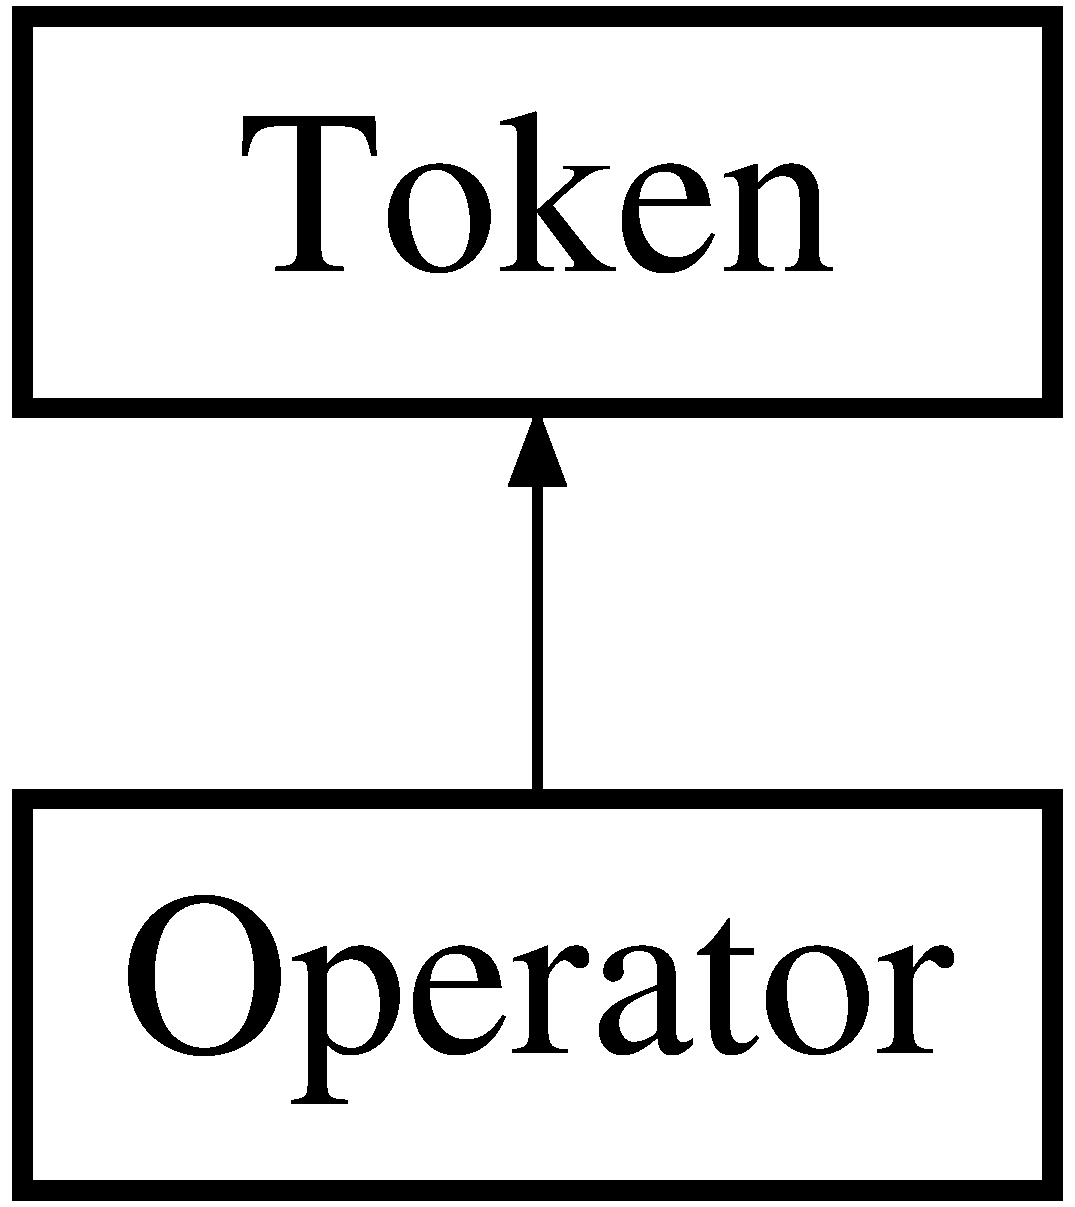
\includegraphics[height=2.000000cm]{d4/dad/classOperator}
\end{center}
\end{figure}
\subsection*{Fungsi Anggota Publik}
\begin{DoxyCompactItemize}
\item 
\hypertarget{classOperator_a2199e61dda5314db8401081f2178d9a9}{}{\bfseries Operator} (std\+::string \+\_\+s)\label{classOperator_a2199e61dda5314db8401081f2178d9a9}

\item 
\hypertarget{classOperator_af0113b1134d9e54abd2a05ea69c63238}{}Enum\+Operator {\bfseries Get\+Jenis\+Operator} ()\label{classOperator_af0113b1134d9e54abd2a05ea69c63238}

\item 
\hypertarget{classOperator_a97faadd3b0c23c108eba25c409b0003d}{}std\+::string {\bfseries Display} ()\label{classOperator_a97faadd3b0c23c108eba25c409b0003d}

\item 
\hypertarget{classOperator_a52745643d188234ebac14062af0fb69c}{}Enum\+Type {\bfseries Get\+Type} ()\label{classOperator_a52745643d188234ebac14062af0fb69c}

\end{DoxyCompactItemize}
\subsection*{Atribut Publik Statis}
\begin{DoxyCompactItemize}
\item 
\hypertarget{classOperator_a932146b92cb0b726be4ec8674af116f4}{}static std\+::string {\bfseries Karakter\+Operator} \mbox{[}$\,$\mbox{]}\label{classOperator_a932146b92cb0b726be4ec8674af116f4}

\item 
\hypertarget{classOperator_a8064c68677326d96415034012d90ba7d}{}static int {\bfseries Banyak\+Operator}\label{classOperator_a8064c68677326d96415034012d90ba7d}

\end{DoxyCompactItemize}
\subsection*{Atribut Privat}
\begin{DoxyCompactItemize}
\item 
\hypertarget{classOperator_af84004b1a9a08a7595350895a4083fcf}{}Enum\+Operator {\bfseries Jenis\+Operator}\label{classOperator_af84004b1a9a08a7595350895a4083fcf}

\end{DoxyCompactItemize}


\subsection{Keterangan Lengkap}
Class \hyperlink{classOperator}{Operator}. 

Kelas yang digunakan untuk merepresentasikan token operator 

Dokumentasi untuk kelas ini dibangkitkan dari file berikut\+:\begin{DoxyCompactItemize}
\item 
/home/ibrohim/oop002/Operator.\+h\end{DoxyCompactItemize}

\hypertarget{classParser}{}\section{Referensi Kelas Parser}
\label{classParser}\index{Parser@{Parser}}


Class \hyperlink{classParser}{Parser}.  


\subsection*{Fungsi Anggota Publik}
\begin{DoxyCompactItemize}
\item 
\hypertarget{classParser_a44fc8feda2b68b7bfcba5a3d1a60df8c}{}void {\bfseries Set\+Mode\+Bilangan} (Enum\+Bilangan B)\label{classParser_a44fc8feda2b68b7bfcba5a3d1a60df8c}

\item 
\hypertarget{classParser_a9241f5ed7a2c1959ed0bbb6f333d30eb}{}\hyperlink{classExpression}{Expression} {\bfseries Parse} (const std\+::string \&s)\label{classParser_a9241f5ed7a2c1959ed0bbb6f333d30eb}

\end{DoxyCompactItemize}
\subsection*{Atribut Privat}
\begin{DoxyCompactItemize}
\item 
\hypertarget{classParser_a171d8521ead0a5726fe262e410f6d970}{}Enum\+Bilangan {\bfseries Mode\+B}\label{classParser_a171d8521ead0a5726fe262e410f6d970}

\end{DoxyCompactItemize}


\subsection{Keterangan Lengkap}
Class \hyperlink{classParser}{Parser}. 

Kelas yang digunakan untuk melakukan proses parsing string 

Dokumentasi untuk kelas ini dibangkitkan dari file berikut\+:\begin{DoxyCompactItemize}
\item 
/home/ibrohim/oop002/Parser.\+h\end{DoxyCompactItemize}

\hypertarget{classParserException}{}\section{Referensi Kelas Parser\+Exception}
\label{classParserException}\index{Parser\+Exception@{Parser\+Exception}}
\subsection*{Fungsi Anggota Publik}
\begin{DoxyCompactItemize}
\item 
\hypertarget{classParserException_a73e9c79df9bacd24553686e317461a18}{}{\bfseries Parser\+Exception} (const std\+::string \&s)\label{classParserException_a73e9c79df9bacd24553686e317461a18}

\item 
\hypertarget{classParserException_a67db03e39544827abd7a5d94a09818ec}{}void {\bfseries Display\+Msg} ()\label{classParserException_a67db03e39544827abd7a5d94a09818ec}

\end{DoxyCompactItemize}


Dokumentasi untuk kelas ini dibangkitkan dari file berikut\+:\begin{DoxyCompactItemize}
\item 
/home/ibrohim/oop002/Parser\+Exception.\+h\end{DoxyCompactItemize}

\hypertarget{classPenghitung}{}\section{Referensi Kelas Penghitung}
\label{classPenghitung}\index{Penghitung@{Penghitung}}


Class \hyperlink{classPenghitung}{Penghitung}.  




{\ttfamily \#include \char`\"{}Penghitung.\+h\char`\"{}}

\subsection*{Fungsi Anggota Publik}
\begin{DoxyCompactItemize}
\item 
\hypertarget{classPenghitung_a131a947d8e8271a40c06617b537719bf}{}{\bfseries Penghitung} (const \hyperlink{classPenghitung}{Penghitung} \&)\label{classPenghitung_a131a947d8e8271a40c06617b537719bf}

\item 
\hypertarget{classPenghitung_a89d5dbc2ba4990d20cbd23b8dc36e5d8}{}double {\bfseries Calculate} (\hyperlink{classExpression}{Expression})\label{classPenghitung_a89d5dbc2ba4990d20cbd23b8dc36e5d8}

\item 
\hypertarget{classPenghitung_aa47317ed3b4985c8fb59ac2695db4c56}{}void {\bfseries Set\+Sintaks} (Enum\+Sintaks)\label{classPenghitung_aa47317ed3b4985c8fb59ac2695db4c56}

\item 
\hypertarget{classPenghitung_ac810fdb8a3c14ce1eada51519830d624}{}void {\bfseries Set\+Math\+Logic} (Enum\+Math\+Logic)\label{classPenghitung_ac810fdb8a3c14ce1eada51519830d624}

\item 
\hypertarget{classPenghitung_a341680e8cf1b3d885bcf033595f124eb}{}double {\bfseries Calculate\+Postfix} (\hyperlink{classExpression}{Expression} \&)\label{classPenghitung_a341680e8cf1b3d885bcf033595f124eb}

\item 
\hypertarget{classPenghitung_a9a79a76c40718775b4e7bb0da7e398b8}{}void {\bfseries Parse\+Infix} (\hyperlink{classExpression}{Expression} \&)\label{classPenghitung_a9a79a76c40718775b4e7bb0da7e398b8}

\item 
\hypertarget{classPenghitung_acda85405d8d4a66e9b32d79d493c36d6}{}void {\bfseries Parse\+Prefix} (\hyperlink{classExpression}{Expression} \&)\label{classPenghitung_acda85405d8d4a66e9b32d79d493c36d6}

\item 
\hypertarget{classPenghitung_a286c8a27a702a9b07bbb4b226e91c815}{}double {\bfseries Calculate\+Atom} (double, double, \hyperlink{classOperator}{Operator} $\ast$)\label{classPenghitung_a286c8a27a702a9b07bbb4b226e91c815}

\end{DoxyCompactItemize}
\subsection*{Atribut Privat}
\begin{DoxyCompactItemize}
\item 
\hypertarget{classPenghitung_ae43b518225f5e7214ba8a06f8a13fb0d}{}Enum\+Sintaks {\bfseries Mode\+Sintaks}\label{classPenghitung_ae43b518225f5e7214ba8a06f8a13fb0d}

\item 
\hypertarget{classPenghitung_ada6a61b4abe04793864ef38a9b496736}{}Enum\+Math\+Logic {\bfseries Mode\+Math\+Logic}\label{classPenghitung_ada6a61b4abe04793864ef38a9b496736}

\end{DoxyCompactItemize}


\subsection{Keterangan Lengkap}
Class \hyperlink{classPenghitung}{Penghitung}. 

Kelas yang digunakan untuk melakukan proses menghitung token 

Dokumentasi untuk kelas ini dibangkitkan dari file berikut\+:\begin{DoxyCompactItemize}
\item 
/home/ibrohim/oop002/Penghitung.\+h\end{DoxyCompactItemize}

\hypertarget{classPenghitungException}{}\section{Referensi Kelas Penghitung\+Exception}
\label{classPenghitungException}\index{Penghitung\+Exception@{Penghitung\+Exception}}


Class \hyperlink{classPenghitungException}{Penghitung\+Exception}.  




{\ttfamily \#include \char`\"{}Penghitung\+Exception.\+h\char`\"{}}

\subsection*{Fungsi Anggota Publik}
\begin{DoxyCompactItemize}
\item 
\hypertarget{classPenghitungException_a988a376427f299e37cc8812497a0f0d4}{}{\bfseries Penghitung\+Exception} (const std\+::string \&s)\label{classPenghitungException_a988a376427f299e37cc8812497a0f0d4}

\item 
\hypertarget{classPenghitungException_aac32ab678c77a1b69229d89e6ed77405}{}void {\bfseries Display\+Msg} ()\label{classPenghitungException_aac32ab678c77a1b69229d89e6ed77405}

\end{DoxyCompactItemize}


\subsection{Keterangan Lengkap}
Class \hyperlink{classPenghitungException}{Penghitung\+Exception}. 

Dokumentasi untuk kelas ini dibangkitkan dari file berikut\+:\begin{DoxyCompactItemize}
\item 
/home/ibrohim/oop002/Penghitung\+Exception.\+h\end{DoxyCompactItemize}

\hypertarget{classPerintah}{}\section{Referensi Kelas Perintah}
\label{classPerintah}\index{Perintah@{Perintah}}


Class \hyperlink{classPerintah}{Perintah}.  




{\ttfamily \#include \char`\"{}Perintah.\+h\char`\"{}}

Diagram hierarki kelas untuk Perintah\+:\begin{figure}[H]
\begin{center}
\leavevmode
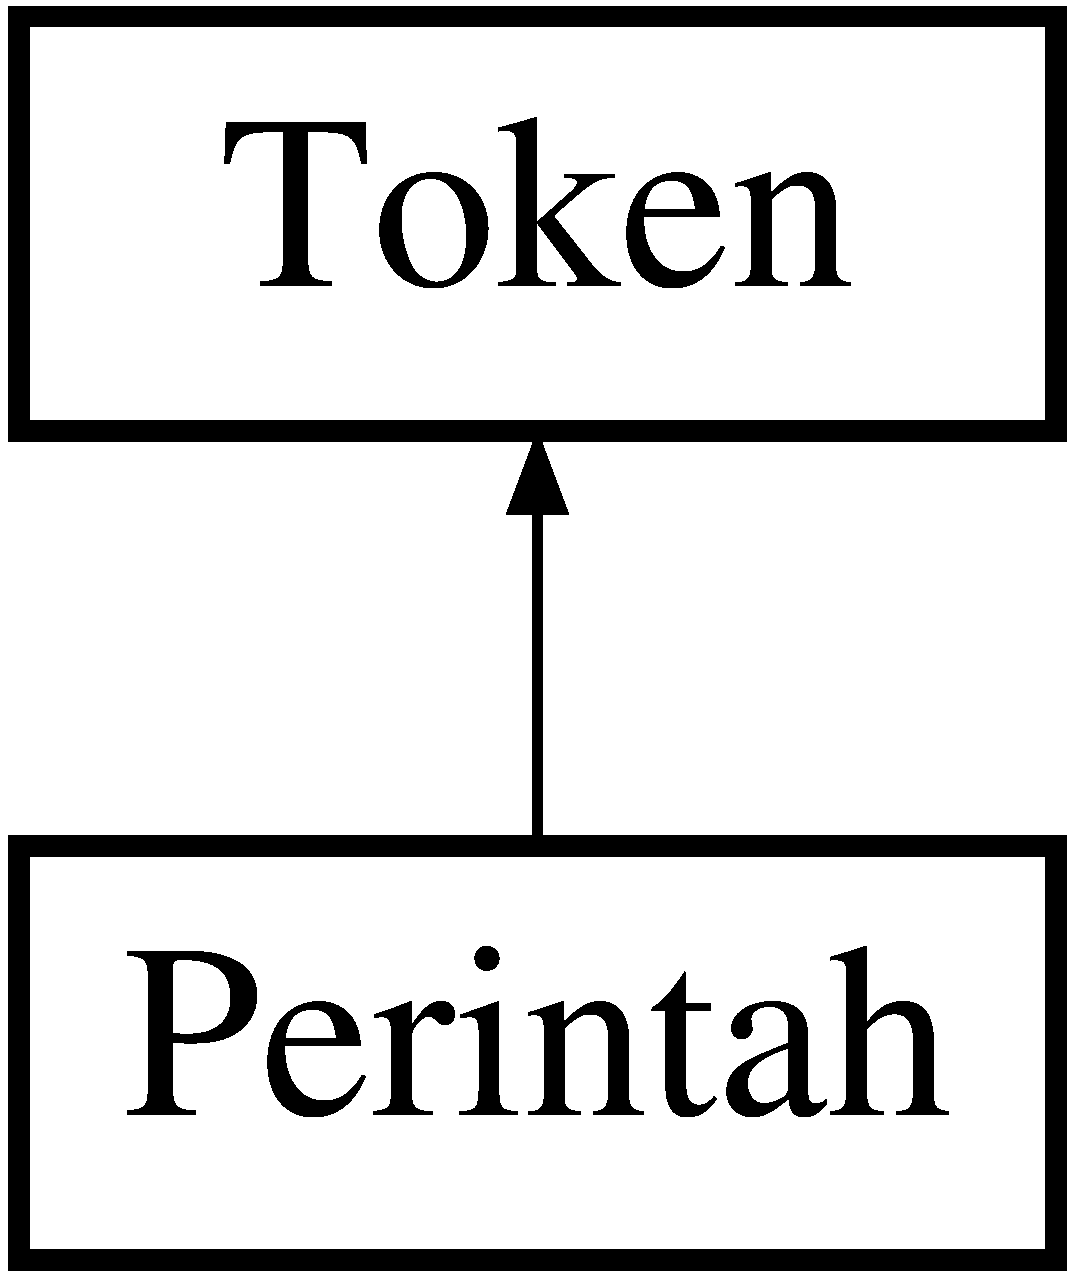
\includegraphics[height=2.000000cm]{d9/de7/classPerintah}
\end{center}
\end{figure}
\subsection*{Fungsi Anggota Publik}
\begin{DoxyCompactItemize}
\item 
\hypertarget{classPerintah_a653750ef3a98a12a11b3bfb6285484c2}{}{\bfseries Perintah} (std\+::string \+\_\+s)\label{classPerintah_a653750ef3a98a12a11b3bfb6285484c2}

\item 
\hypertarget{classPerintah_aef16391fc67acc7ff74354db10eaa92a}{}Enum\+Perintah {\bfseries Get\+Jenis\+Perintah} ()\label{classPerintah_aef16391fc67acc7ff74354db10eaa92a}

\item 
\hypertarget{classPerintah_a32e0674e117dea6e1b69ea66ed885ea1}{}std\+::string {\bfseries Display} ()\label{classPerintah_a32e0674e117dea6e1b69ea66ed885ea1}

\item 
\hypertarget{classPerintah_ad2e51be1b5d590c538be4eeaecd9b110}{}Enum\+Type {\bfseries Get\+Type} ()\label{classPerintah_ad2e51be1b5d590c538be4eeaecd9b110}

\end{DoxyCompactItemize}
\subsection*{Atribut Publik Statis}
\begin{DoxyCompactItemize}
\item 
\hypertarget{classPerintah_ad52acf87f08dae5f2756e80597a925e5}{}static std\+::string {\bfseries Karakter\+Perintah} \mbox{[}$\,$\mbox{]}\label{classPerintah_ad52acf87f08dae5f2756e80597a925e5}

\item 
\hypertarget{classPerintah_afb3b32fca72ced1dd39c9083d65f721e}{}static int {\bfseries Banyak\+Perintah}\label{classPerintah_afb3b32fca72ced1dd39c9083d65f721e}

\end{DoxyCompactItemize}


\subsection{Keterangan Lengkap}
Class \hyperlink{classPerintah}{Perintah}. 

Dokumentasi untuk kelas ini dibangkitkan dari file berikut\+:\begin{DoxyCompactItemize}
\item 
/home/ibrohim/oop002/Perintah.\+h\end{DoxyCompactItemize}

\hypertarget{classRomawi}{}\section{Referensi Kelas Romawi}
\label{classRomawi}\index{Romawi@{Romawi}}


Class \hyperlink{classRomawi}{Romawi}.  




{\ttfamily \#include \char`\"{}Romawi.\+h\char`\"{}}

Diagram hierarki kelas untuk Romawi\+:\begin{figure}[H]
\begin{center}
\leavevmode
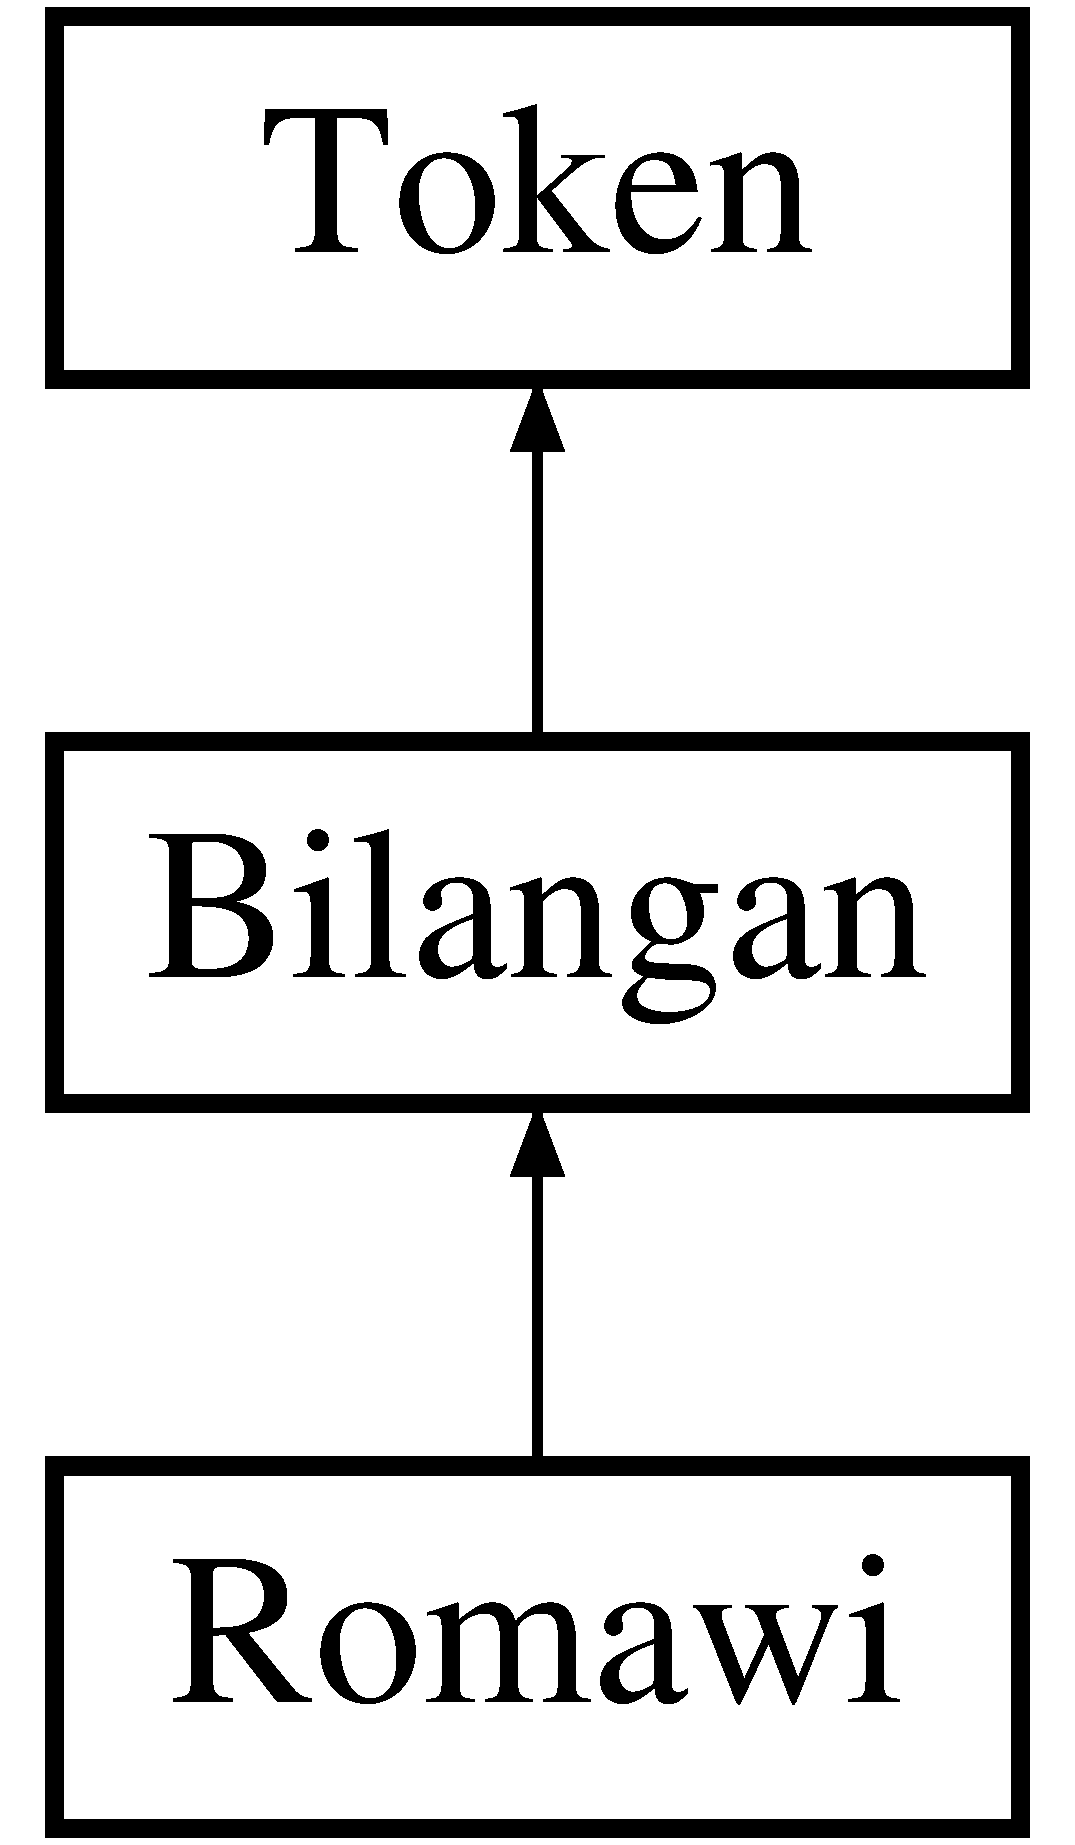
\includegraphics[height=3.000000cm]{d9/de3/classRomawi}
\end{center}
\end{figure}
\subsection*{Fungsi Anggota Publik}
\begin{DoxyCompactItemize}
\item 
\hypertarget{classRomawi_ad246367c51d3d67d4fbaaee36031ccd1}{}{\bfseries Romawi} (const double d)\label{classRomawi_ad246367c51d3d67d4fbaaee36031ccd1}

\item 
\hypertarget{classRomawi_a46332c134c2f38feb7787994bd99e3ad}{}{\bfseries Romawi} (const std\+::string \&s)\label{classRomawi_a46332c134c2f38feb7787994bd99e3ad}

\item 
\hypertarget{classRomawi_adc5a0a8e2ad13902f66da32e5ebe2bfe}{}double {\bfseries Get\+Value} ()\label{classRomawi_adc5a0a8e2ad13902f66da32e5ebe2bfe}

\item 
\hypertarget{classRomawi_a630b1a4635acfaa7a3def12b5a6aaecc}{}std\+::string {\bfseries Display} ()\label{classRomawi_a630b1a4635acfaa7a3def12b5a6aaecc}

\end{DoxyCompactItemize}


\subsection{Keterangan Lengkap}
Class \hyperlink{classRomawi}{Romawi}. 

Dokumentasi untuk kelas ini dibangkitkan dari file berikut\+:\begin{DoxyCompactItemize}
\item 
/home/ibrohim/oop002/Romawi.\+h\end{DoxyCompactItemize}

\hypertarget{classstack}{}\section{Referensi Kelas Template stack$<$ T $>$}
\label{classstack}\index{stack$<$ T $>$@{stack$<$ T $>$}}


Class stack.  




{\ttfamily \#include \char`\"{}S\+T\+L/stack.\+h\char`\"{}}

\subsection*{Fungsi Anggota Publik}
\begin{DoxyCompactItemize}
\item 
\hypertarget{classstack_aa2b7837e7fa4708c17c0a78520d18924}{}{\bfseries stack} (const \hyperlink{classstack}{stack} \&s)\label{classstack_aa2b7837e7fa4708c17c0a78520d18924}

\item 
\hypertarget{classstack_a6c35161825c5a23462f4830a047823bc}{}\hyperlink{classstack}{stack} \& {\bfseries operator=} (const \hyperlink{classstack}{stack}$<$ T $>$ \&s)\label{classstack_a6c35161825c5a23462f4830a047823bc}

\item 
\hypertarget{classstack_ad6615a82d944ce2e9a9c260b1d126666}{}void {\bfseries pop} ()\label{classstack_ad6615a82d944ce2e9a9c260b1d126666}

\item 
\hypertarget{classstack_a532ce58222bf37610dbf90c37b42ba98}{}void {\bfseries push} (T e)\label{classstack_a532ce58222bf37610dbf90c37b42ba98}

\item 
\hypertarget{classstack_a6093fd7036685b3d9ea89e96609465ac}{}T {\bfseries top} ()\label{classstack_a6093fd7036685b3d9ea89e96609465ac}

\item 
\hypertarget{classstack_a1577ac10f88c5d6bdbbd9f8f61344b91}{}int {\bfseries size} ()\label{classstack_a1577ac10f88c5d6bdbbd9f8f61344b91}

\item 
\hypertarget{classstack_ab82d4f94c3a83318499848de576feede}{}bool {\bfseries empty} ()\label{classstack_ab82d4f94c3a83318499848de576feede}

\end{DoxyCompactItemize}


\subsection{Keterangan Lengkap}
\subsubsection*{template$<$class T$>$class stack$<$ T $>$}

Class stack. 

Dokumentasi untuk kelas ini dibangkitkan dari file berikut\+:\begin{DoxyCompactItemize}
\item 
/home/ibrohim/oop002/\+S\+T\+L/stack.\+h\end{DoxyCompactItemize}

\hypertarget{classStackExp}{}\section{Referensi Kelas Stack\+Exp}
\label{classStackExp}\index{Stack\+Exp@{Stack\+Exp}}
\subsection*{Fungsi Anggota Publik}
\begin{DoxyCompactItemize}
\item 
\hypertarget{classStackExp_a2590e6d22201f3c187d83bf9e626b6e2}{}{\bfseries Stack\+Exp} (int e)\label{classStackExp_a2590e6d22201f3c187d83bf9e626b6e2}

\item 
\hypertarget{classStackExp_a8d3e08d13c04cd4577899971cbda6094}{}void {\bfseries print\+Msg} ()\label{classStackExp_a8d3e08d13c04cd4577899971cbda6094}

\end{DoxyCompactItemize}


Dokumentasi untuk kelas ini dibangkitkan dari file berikut\+:\begin{DoxyCompactItemize}
\item 
/home/ibrohim/oop002/\+S\+T\+L/stack.\+h\end{DoxyCompactItemize}

\hypertarget{classToken}{}\section{Referensi Kelas Token}
\label{classToken}\index{Token@{Token}}


Class \hyperlink{classToken}{Token}.  




{\ttfamily \#include \char`\"{}Token.\+h\char`\"{}}

Diagram hierarki kelas untuk Token\+:\begin{figure}[H]
\begin{center}
\leavevmode
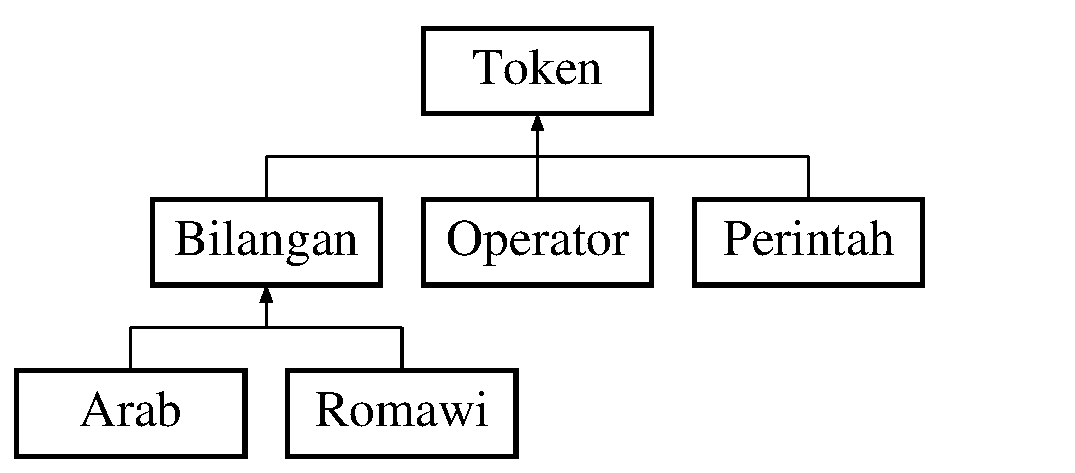
\includegraphics[height=3.000000cm]{d2/d6e/classToken}
\end{center}
\end{figure}
\subsection*{Fungsi Anggota Publik}
\begin{DoxyCompactItemize}
\item 
\hypertarget{classToken_a86f97e77bdba8277b58ead29d3ef3584}{}virtual Enum\+Type {\bfseries Get\+Type} ()=0\label{classToken_a86f97e77bdba8277b58ead29d3ef3584}

\item 
\hypertarget{classToken_a89fa3f496f16d14fcf4b4f1a4047229b}{}virtual std\+::string {\bfseries Display} ()=0\label{classToken_a89fa3f496f16d14fcf4b4f1a4047229b}

\end{DoxyCompactItemize}


\subsection{Keterangan Lengkap}
Class \hyperlink{classToken}{Token}. 

Dokumentasi untuk kelas ini dibangkitkan dari file berikut\+:\begin{DoxyCompactItemize}
\item 
/home/ibrohim/oop002/Token.\+h\end{DoxyCompactItemize}

\hypertarget{classvector}{}\section{Referensi Kelas Template vector$<$ T $>$}
\label{classvector}\index{vector$<$ T $>$@{vector$<$ T $>$}}


Class vector.  




{\ttfamily \#include \char`\"{}S\+T\+L/vector.\+h\char`\"{}}

\subsection*{Fungsi Anggota Publik}
\begin{DoxyCompactItemize}
\item 
\hypertarget{classvector_ae0d26803a00988f33ca95a5a53d11c54}{}{\bfseries vector} (unsigned int size)\label{classvector_ae0d26803a00988f33ca95a5a53d11c54}

\item 
\hypertarget{classvector_a397ada02bf67d465821ba54d07e47e0c}{}{\bfseries vector} (unsigned int size, const T \&initial)\label{classvector_a397ada02bf67d465821ba54d07e47e0c}

\item 
\hypertarget{classvector_ae95f31bd9366f4af589095346962679f}{}{\bfseries vector} (const \hyperlink{classvector}{vector}$<$ T $>$ \&v)\label{classvector_ae95f31bd9366f4af589095346962679f}

\item 
\hypertarget{classvector_ac68f7da6ca40206d8fbfdd80c3b12b62}{}unsigned int {\bfseries capacity} () const \label{classvector_ac68f7da6ca40206d8fbfdd80c3b12b62}

\item 
\hypertarget{classvector_abd541636a83700f5708ee109fca6796a}{}unsigned int {\bfseries size} () const \label{classvector_abd541636a83700f5708ee109fca6796a}

\item 
\hypertarget{classvector_a6c885f006c9b70e0533e7194f5ae70a0}{}bool {\bfseries empty} () const \label{classvector_a6c885f006c9b70e0533e7194f5ae70a0}

\item 
\hypertarget{classvector_ad76deb64969b591fe8accbd2f69ea271}{}void {\bfseries push\+\_\+back} (const T \&value)\label{classvector_ad76deb64969b591fe8accbd2f69ea271}

\item 
\hypertarget{classvector_aeec9e5d602d555d466a936310aa47866}{}void {\bfseries pop\+\_\+back} ()\label{classvector_aeec9e5d602d555d466a936310aa47866}

\item 
\hypertarget{classvector_ae37ac6075980a3113fc442ce4411204c}{}void {\bfseries reserve} (unsigned int capacity)\label{classvector_ae37ac6075980a3113fc442ce4411204c}

\item 
\hypertarget{classvector_a313d7dd651ab48eeddf7845cbd5bc5af}{}void {\bfseries resize} (unsigned int size)\label{classvector_a313d7dd651ab48eeddf7845cbd5bc5af}

\item 
\hypertarget{classvector_ab6ebd10d627f8eb33e15c27cf7aaf36a}{}T \& {\bfseries operator\mbox{[}$\,$\mbox{]}} (unsigned int index) const \label{classvector_ab6ebd10d627f8eb33e15c27cf7aaf36a}

\item 
\hypertarget{classvector_ad88d3a7709894cdb0b471db0a7a8eb6f}{}\hyperlink{classvector}{vector}$<$ T $>$ \& {\bfseries operator=} (const \hyperlink{classvector}{vector}$<$ T $>$ \&)\label{classvector_ad88d3a7709894cdb0b471db0a7a8eb6f}

\item 
\hypertarget{classvector_a1a91cd18e54c382af1097d630405398f}{}void {\bfseries clear} ()\label{classvector_a1a91cd18e54c382af1097d630405398f}

\end{DoxyCompactItemize}
\subsection*{Atribut Privat}
\begin{DoxyCompactItemize}
\item 
\hypertarget{classvector_adc0382744358059c7ed8c9315ea691aa}{}unsigned int {\bfseries \+\_\+size}\label{classvector_adc0382744358059c7ed8c9315ea691aa}

\item 
\hypertarget{classvector_a1c2a061959c956eb85805934b00ad75d}{}unsigned int {\bfseries \+\_\+capacity}\label{classvector_a1c2a061959c956eb85805934b00ad75d}

\item 
\hypertarget{classvector_a71e90789f12e267399ac7387521cc548}{}unsigned int {\bfseries Log}\label{classvector_a71e90789f12e267399ac7387521cc548}

\item 
\hypertarget{classvector_adb51efa5b9d82cddfa401836401bb8f1}{}T $\ast$ {\bfseries buffer}\label{classvector_adb51efa5b9d82cddfa401836401bb8f1}

\end{DoxyCompactItemize}


\subsection{Keterangan Lengkap}
\subsubsection*{template$<$class T$>$class vector$<$ T $>$}

Class vector. 

Kelas vector yang diimplementasi berdasarkan \hyperlink{namespaceSTL}{S\+T\+L} C++ 

Dokumentasi untuk kelas ini dibangkitkan dari file berikut\+:\begin{DoxyCompactItemize}
\item 
/home/ibrohim/oop002/\+S\+T\+L/vector.\+h\end{DoxyCompactItemize}

%--- End generated contents ---

% Index
\backmatter
\newpage
\phantomsection
\clearemptydoublepage
\addcontentsline{toc}{chapter}{Indeks}
\printindex

\end{document}
